\documentclass[11pt]{article}

\usepackage[utf8]{inputenc}
\usepackage[T1]{fontenc}
\usepackage{graphicx}
\usepackage{booktabs}
\usepackage{amsmath}
\usepackage{siunitx}
\usepackage[hidelinks]{hyperref}
\usepackage[round]{natbib}
\usepackage{geometry}
\geometry{margin=1in}

% Figures are produced by the analysis pipeline into ../results/figures/
\graphicspath{{../results/figures/}}

\title{Inferring the Potentially-Hazardous Status of Near-Earth Objects from
Observed Close-Approach Kinematics: A Selection-Aware, Leakage-Controlled Study}

\author{J.\ Yukopila \and D.\ Garcia \and C.\ Toro}
\date{\today}

\begin{document}
\maketitle

\begin{abstract}
Machine-learning classifiers routinely separate Potentially Hazardous Asteroids
(PHAs) from other near-Earth objects (NEOs) with near-perfect scores. We argue that
much of this success is circular: the PHA label is, by definition, a deterministic
threshold on the minimum orbit intersection distance (MOID) and absolute magnitude
$H$, so feeding those quantities to a model amounts to relearning the defining rule.
We instead ask a harder question: can hazard be inferred from the \emph{observed}
close-approach kinematics alone---without the orbital elements that define it---and
how is that inference shaped by the survey selection function imprinted on a
126-year close-approach catalog? Using a self-collected catalog of
\num{32568} close-approach events for \num{18934} unique NEOs (JPL/CNEOS), labeled
with the official JPL Small-Body Database PHA flag, we show that (i) a two-threshold
rule on observed quantities matches gradient-boosted trees ($F_2\approx0.98$),
confirming the circularity; (ii) the predictive signal is carried almost entirely by
object \emph{size}, not by kinematics---removing size collapses $F_2$ to
$\sim$\,0.2--0.5; and (iii) PHA prevalence falls monotonically from $\sim$95\% to
$\sim$1\% with discovery epoch, tracked by orbital arc length, demonstrating that the
catalog is a detection record rather than a census. We provide a reproducible,
selection-aware protocol and a frozen data snapshot.
\end{abstract}

\section{Introduction}
Near-Earth objects that can make close approaches to Earth are monitored for impact
risk. The operational hazard category, the Potentially Hazardous Asteroid (PHA), is
defined by two thresholds: a minimum orbit intersection distance $\mathrm{MOID}\le
0.05$~au \emph{and} an absolute magnitude $H\le 22$ (diameter $\gtrsim 140$~m)
\citep{cneos_pha}. A large applied-ML literature trains classifiers to predict this
flag, typically reporting 98--99\% accuracy with random forests, gradient boosting,
or graph neural networks \citep{neo_resampling2025,neo_gnn2025,neo_xai2025}. Because
the standard feature sets include MOID and $H$---the very quantities that
\emph{define} the label---such models largely relearn a closed-form rule, an effect
amounting to target leakage rather than scientific prediction. The widely used
benchmark of \citet{kaggle_neo} is essentially close-approach data (miss distance,
relative velocity, $H$, diameter, hazard flag) without orbital elements or epochs.

We reframe the task. Our catalog contains only \emph{observed} close-approach
geometry---no orbital elements---plus, crucially, time stamps spanning 1900--2026 and
multiple approaches per object. We therefore ask whether hazard can be inferred from
observed kinematics alone, and we quantify the observational selection function that
any such inference inherits. Our contributions are: (1) a leakage-controlled
formulation that excludes the defining orbital elements; (2) explicit evidence that
the apparent ``predictability'' of PHAs is circular and size-driven; (3) a
selection-aware temporal analysis, keyed to the real first-observation date, that
exposes how survey growth reshapes the labeled population; and (4) a fully
reproducible pipeline with a frozen, dated data snapshot.

\section{Related Work}
Supervised PHA classification has been studied with resampling strategies for class
imbalance \citep{neo_resampling2025}, explainable AI and anomaly detection
\citep{neo_xai2025}, and graph neural networks that report AUC$\approx$0.99 on a
catalog with only 0.22\% hazardous objects \citep{neo_gnn2025}. These works
consistently (a) include MOID and $H$ as features, (b) treat the catalog as a static
sample, and (c) emphasize accuracy/AUC. We depart from all three: we withhold the
defining orbital elements, treat the catalog as a time-evolving detection record, and
report imbalance-appropriate metrics with cross-validated intervals.

\section{Data}
We query the CNEOS Close-Approach Data (CAD) API \citep{cneos_cad} for all close
approaches from 1900 to the query date with estimated diameters, and the JPL
Small-Body Database (SBDB) query API \citep{jpl_sbdb} for the official \texttt{pha}
flag, MOID, $H$, first-observation date, and orbital data arc. Matching CAD
designations to SBDB primary designations succeeds for 99.9\% of objects (unmatched
cases are comets). The frozen snapshot used here
(\texttt{close\_approaches\_v20260619.csv}) contains \num{32568} events for
\num{18934} objects; \num{18927} are matched and labeled, with a PHA prevalence of
7.3\%.

\paragraph{Unit of analysis and labels.}
Hazard is a property of an \emph{object}, so we aggregate events per designation
(minimum observed approach distance, maximum/median velocities, minimum $H$, maximum
diameter, number of approaches, first-observation year, orbital arc). The target is
the official PHA flag. As a self-contained sanity check we also derive a
\emph{proxy} label from observed quantities only ($H\le 22$ and minimum observed
$\mathrm{dist\_min}\le 0.05$~au); it reproduces the official flag with precision
0.966 and recall 0.984. The observed minimum distance approximates MOID with
$r\approx0.73$ (Fig.~\ref{fig:moid}); the gap is physical---one rarely observes the
closest geometrically possible approach---so the observed distance is biased high
relative to MOID.

\paragraph{Caveat: imputation.}
Where diameters are missing, CAD imputes them from $H$ via the standard albedo
relation, making $H$ and diameter partly deterministic; we account for this in
feature pruning.

\section{Methods}
\paragraph{Feature pruning.}
Object-level features are strongly collinear (Fig.~\ref{fig:collinear}): the three
velocity summaries are nearly identical ($|r|\approx1.0$) and the two distance
summaries have $|r|=0.97$. We therefore use pruned sets: \textbf{kin+size}
$=\{\mathrm{dist\_min},\, v_\mathrm{rel},\, H,\, n_\mathrm{appro}\}$, \textbf{kin-only}
$=\{\mathrm{dist\_min},\, v_\mathrm{rel},\, n_\mathrm{appro}\}$, and \textbf{size-only}
$=\{H\}$. No orbital element (MOID, $a$, $e$, $i$) is ever used as a predictor.

\paragraph{Models and evaluation.}
We compare logistic regression, random forests, and XGBoost \citep{xgboost,scikit-learn},
all with class-imbalance handling (balanced class weights or
\texttt{scale\_pos\_weight}). We report $F_2$ (recall-weighted; missing a PHA is
costlier than a false alarm), PR-AUC, and ROC-AUC under repeated stratified
5-fold cross-validation (3 repeats), as mean $\pm$ standard deviation. The decision
threshold is selected to maximize $F_2$ from the out-of-fold precision--recall curve
rather than fixed at 0.5. All runs use a fixed random seed.

\paragraph{Circularity and selection probes.}
We compare every model against a trivial two-threshold rule on observed quantities. We
analyze selection by stratifying on the real first-observation date and by relating
PHA prevalence to orbital arc length (a proxy for how well an object is
characterized). Feature attributions use SHAP \citep{shap}.

\section{Results}

\begin{table}[t]
\centering
\caption{Cross-validated performance (repeated stratified 5-fold, 3 repeats; mean).
Removing size (kin-only) collapses performance; size alone nearly matches the full
set. The trivial threshold rule matches the best models.}
\label{tab:cv}
\begin{tabular}{llccc}
\toprule
Features & Model & $F_2$ & PR-AUC & ROC-AUC \\
\midrule
kin+size  & LogReg     & $0.959\pm0.006$ & 0.956 & 0.998 \\
kin+size  & RandForest & $0.980\pm0.006$ & 0.981 & 0.998 \\
kin+size  & XGBoost    & $0.977\pm0.005$ & 0.987 & 0.999 \\
kin-only  & LogReg     & $0.490\pm0.015$ & 0.308 & 0.840 \\
kin-only  & RandForest & $0.213\pm0.026$ & 0.305 & 0.814 \\
kin-only  & XGBoost    & $0.492\pm0.016$ & 0.351 & 0.842 \\
size-only & LogReg     & $0.956\pm0.007$ & 0.956 & 0.998 \\
size-only & RandForest & $0.970\pm0.008$ & 0.968 & 0.996 \\
size-only & XGBoost    & $0.975\pm0.003$ & 0.974 & 0.999 \\
\midrule
\multicolumn{2}{l}{Threshold rule (dist\_min$\le$0.05 \& $H\le$22)} & 0.980 & --- & --- \\
\bottomrule
\end{tabular}
\end{table}

\paragraph{The task is near-trivial and circular.}
A two-threshold rule on observed quantities achieves $F_2=0.980$ (precision 0.968,
recall 0.983), matching gradient-boosted trees (Table~\ref{tab:cv},
Fig.~\ref{fig:f2}). Reported ``state-of-the-art'' accuracy therefore largely measures
how closely the inputs reproduce the label's definition.

\paragraph{Size, not kinematics, carries the signal.}
Removing size information (kin-only) collapses $F_2$ to 0.2--0.5 and PR-AUC to
$\sim$0.3, whereas size alone ($\{H\}$) nearly matches the full feature set
(Table~\ref{tab:cv}). SHAP and impurity importances concur: $H$ (and the
imputation-linked diameter) dominate, while velocity and distance contribute little
(Fig.~\ref{fig:imp}). Physically, observed proximity alone yields many false
positives---small objects pass close but are not hazardous---so the $H\le22$ size cut
does the discriminative work. The $F_2$-optimal operating threshold is 0.59, not 0.5
(Fig.~\ref{fig:prroc}).

\paragraph{The catalog is a detection record.}
Keying on the real first-observation date, PHA prevalence falls monotonically from
$\sim$95\% for objects discovered before 1990 to 1.3\% for those discovered in the
2020s, while the median orbital arc drops from $\sim$$10^{4}$ days to a few days
(Fig.~\ref{fig:temporal}). Training on objects discovered before 2015
(PHA 23.3\%) and testing on later discoveries (PHA 2.4\%) confirms a large prevalence
shift; PHA status correlates with orbital arc ($r=0.65$), making the characterization
confound explicit. Conditioning the catalog on close approaches only mildly enriches
PHAs relative to all NEOs (7.3\% vs.\ 6.0\%), so the dominant selection is temporal
(discovery), not the close-approach condition itself.

\begin{figure}[t]
\centering
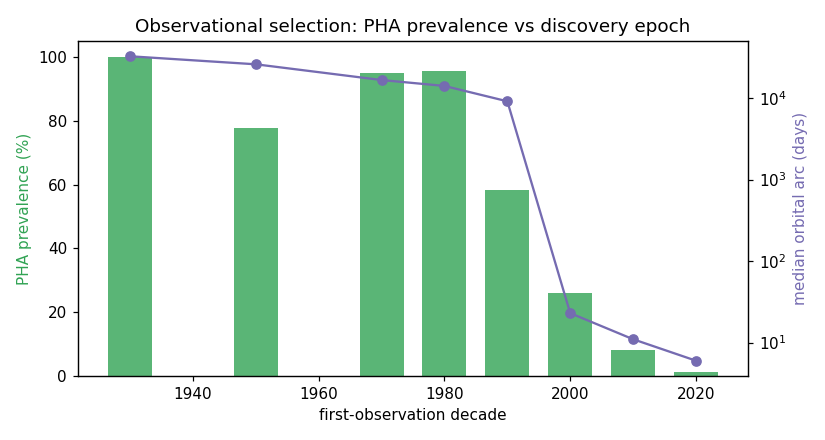
\includegraphics[width=0.8\linewidth]{selection_temporal.png}
\caption{Observational selection. PHA prevalence (bars) versus first-observation
decade, with median orbital arc (line, log scale). Recent surveys add many
small, short-arc, non-hazardous objects.}
\label{fig:temporal}
\end{figure}

\begin{figure}[t]
\centering
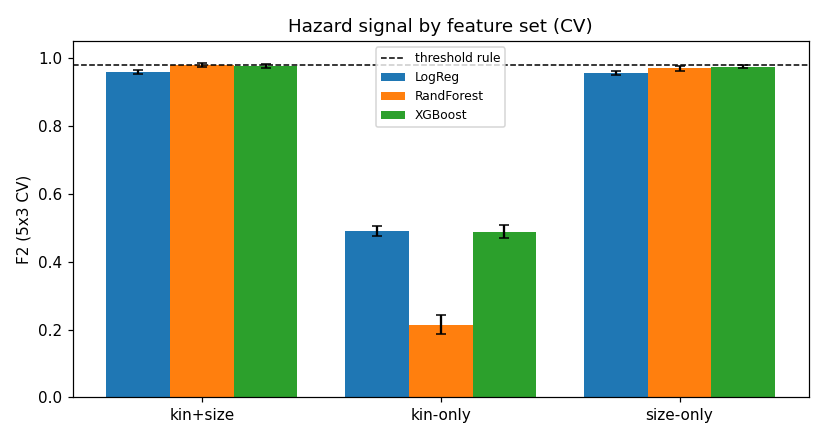
\includegraphics[width=0.85\linewidth]{clf_f2_por_features.png}
\caption{Cross-validated $F_2$ by feature set and model (error bars: CV std). The
dashed line is the trivial threshold rule. kin-only collapses; size-only and
kin+size match the rule.}
\label{fig:f2}
\end{figure}

\begin{figure}[t]
\centering
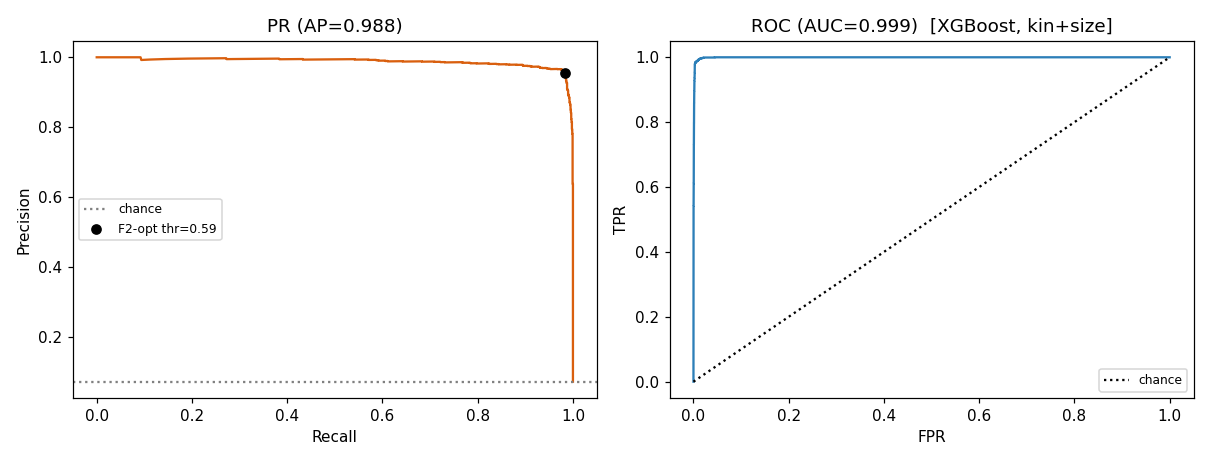
\includegraphics[width=\linewidth]{clf_pr_roc.png}
\caption{Out-of-fold precision--recall (left) and ROC (right) for XGBoost on the
kin+size set, with the $F_2$-optimal operating point.}
\label{fig:prroc}
\end{figure}

\begin{figure}[t]
\centering
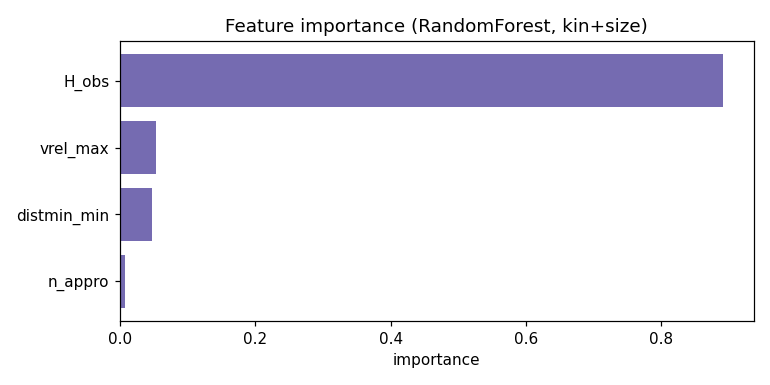
\includegraphics[width=0.7\linewidth]{clf_importancia.png}
\caption{Random-forest feature importances (kin+size). Size ($H$) dominates;
kinematic features are negligible.}
\label{fig:imp}
\end{figure}

\begin{figure}[t]
\centering
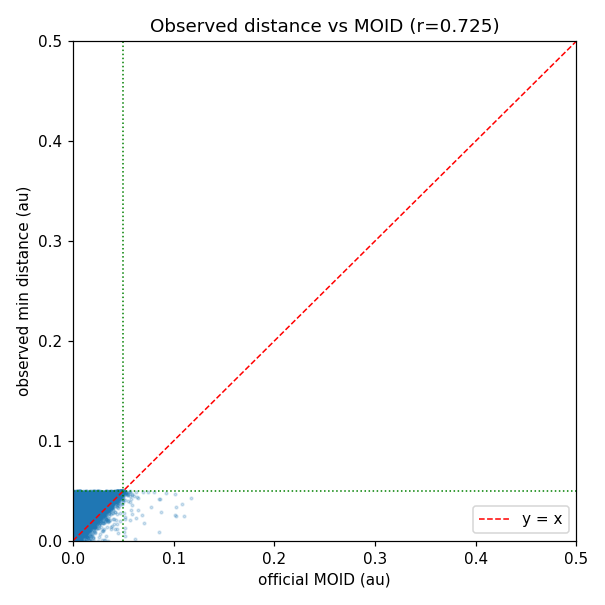
\includegraphics[width=0.55\linewidth]{proxy_vs_moid.png}
\caption{Observed minimum approach distance versus official MOID ($r\approx0.73$).
Points lie above $y=x$: the observed distance is biased high relative to MOID.}
\label{fig:moid}
\end{figure}

\begin{figure}[t]
\centering
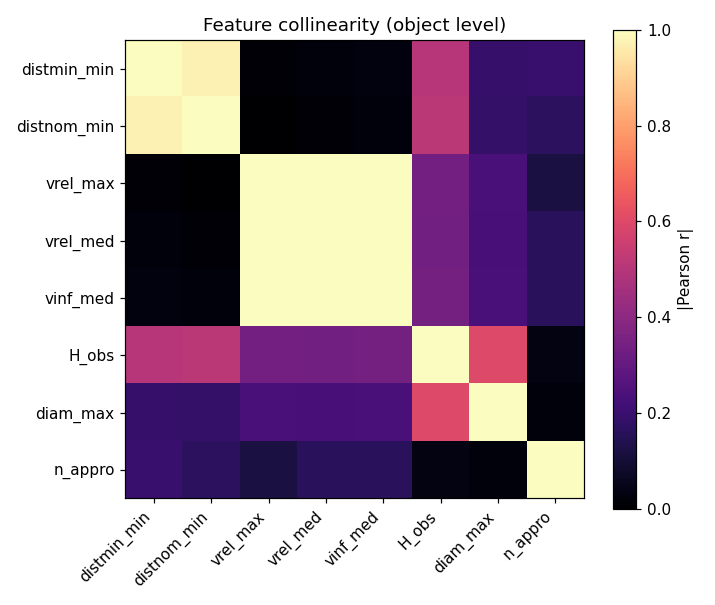
\includegraphics[width=0.6\linewidth]{clf_collinearity.png}
\caption{Absolute Pearson correlation among candidate object-level features,
motivating the pruned sets.}
\label{fig:collinear}
\end{figure}

\section{Discussion}
Our results recast a seemingly solved problem. The high scores in the literature are
real but largely uninformative: they certify that models can reproduce a definition
when given its constituents. When the defining orbital elements are withheld, the
genuine kinematic signal for hazard is weak; what remains is essentially the size
cut. Moreover, the labeled population is not a fixed sample but a moving target shaped
by survey history---an effect invisible to static analyses and directly measurable
here through first-observation date and orbital arc. These observations argue for
selection-aware evaluation (temporal hold-outs, prevalence reporting) in any
applied-ML study built on growing astronomical catalogs.

\section{Limitations}
The catalog is conditioned on objects with catalogued close approaches and on
successful CAD/SBDB cross-matching; missing diameters are imputed from $H$, coupling
two features; and ``observed minimum distance'' is an epoch-limited proxy for MOID.
The temporal axis uses first-observation date, which correlates with orbital arc; we
report both rather than claim a single causal mechanism.

\section{Conclusion}
Inferring PHA status from observed close-approach kinematics alone is hard, and the
easy version of the task is circular. The predictive signal is dominated by size, and
the labeled population is a detection record whose hazard prevalence is set by survey
epoch. We release a reproducible, selection-aware pipeline and a frozen snapshot to
support honest benchmarking. Future work will incorporate orbital elements explicitly
(to study the circularity quantitatively) and extend the analysis to debiased,
completeness-corrected populations.

\paragraph{Data and code availability.}
All code, the headless reproduction driver, and the frozen dated data snapshot are in
the project repository. Figures and the cross-validation results table are
regenerated by a single command.

\paragraph{Author contributions.}
[To be completed by the authors.]

\bibliographystyle{plainnat}
\bibliography{refs}

\end{document}
